\subsection{Communication} \label{subsec:Communication}
The Main Processor and Sample Control modules need a communication interface in order to set control settings for the ADCs, DAC in the FPGA's internal registers and to retrieve stored ADC samples.The ADCs and DAC \todo{Vi mangler at redegøre for det her valg.} both have 16 bits of resolution and a 16 bit wide parallel bus between the FPGA and MCU will be used to transfer the data as shown on figure \refq{fig_7_2_1_CommBus}.

\begin{figure}[H]
    \centering
    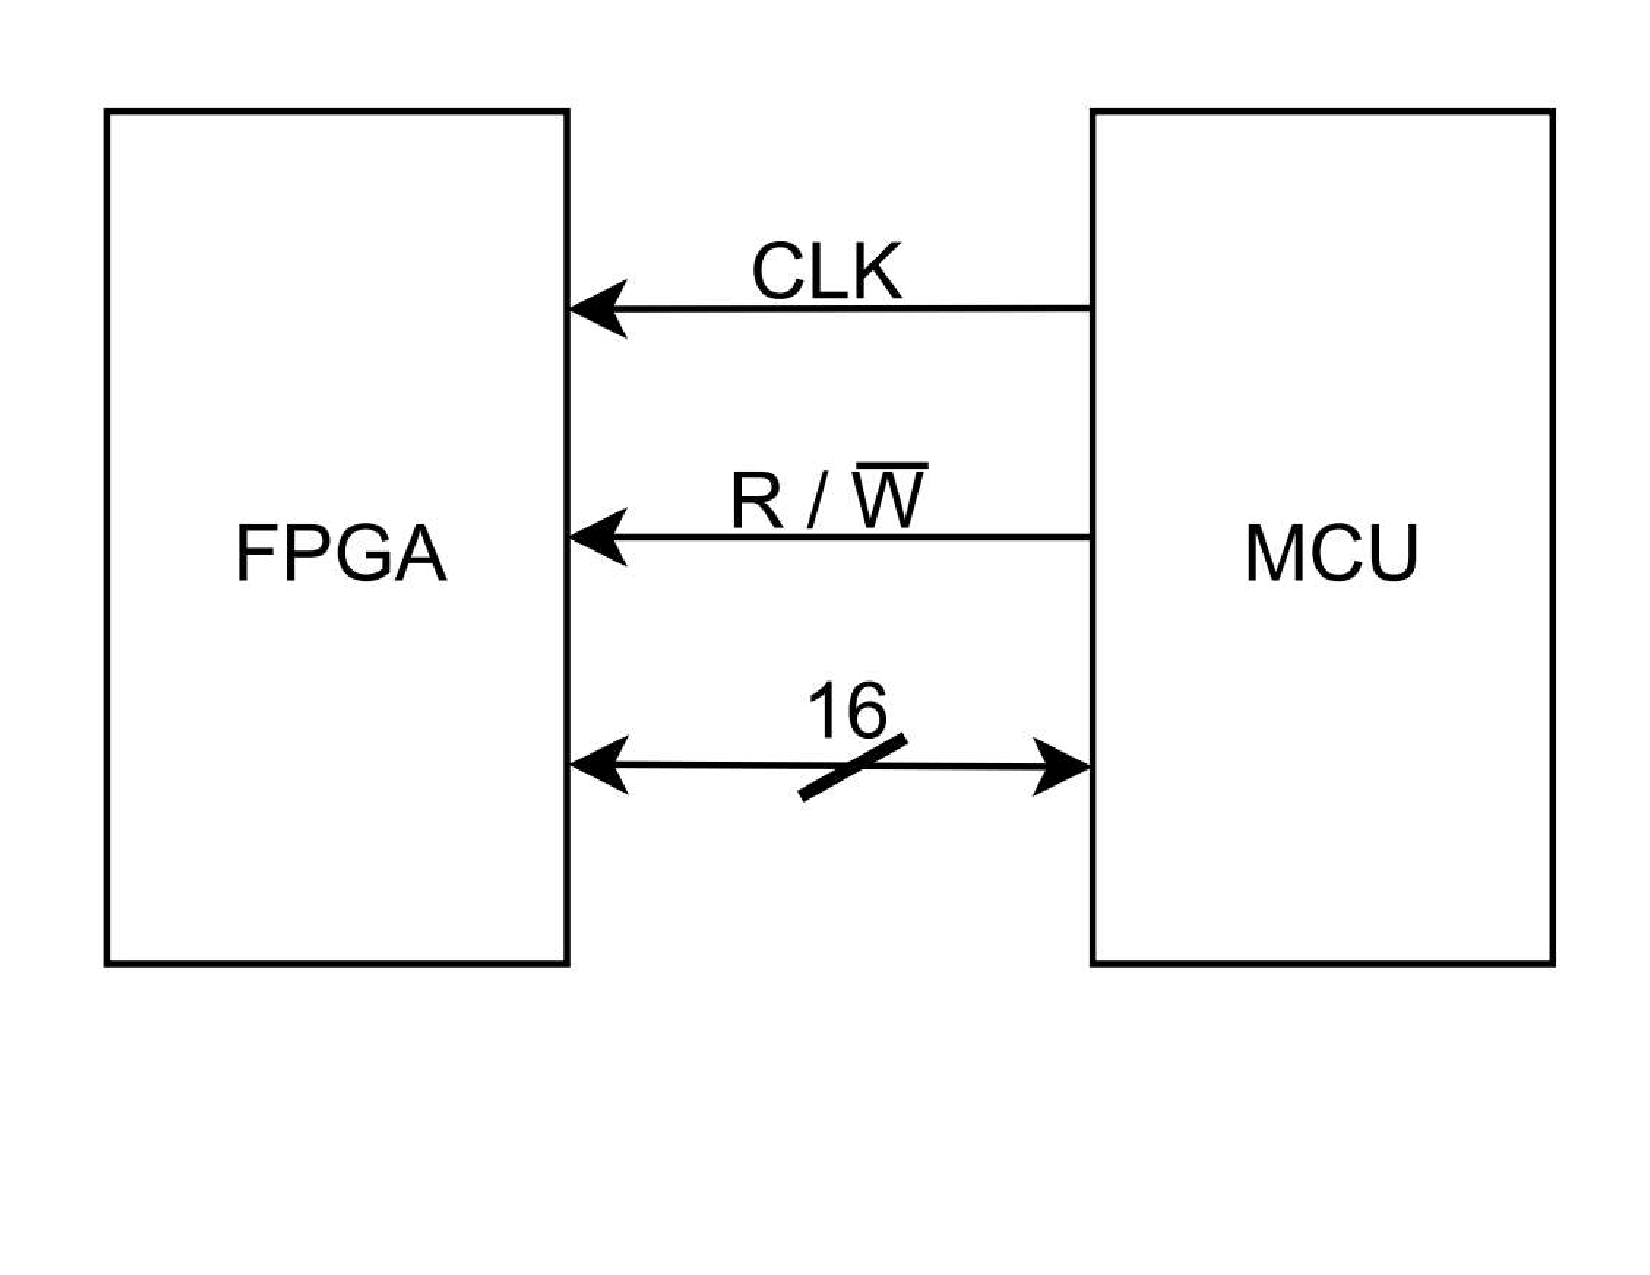
\includegraphics[clip, trim=0 100 0 0, width=0.5\textwidth]{Sections/7_SystemDesign/Figures/7_2_1_CommunicationBus.pdf}
    \caption{The communication bus connection the FPGA and microcontroller. It uses a 16 bit databus, a long with a CLK and a read/write control signal.}
    \label{fig_7_2_1_CommBus}
\end{figure}

The microcontroller is always going to be the master that has to initiate communication and the FPGA is always the slave. The microcontroller is controlling the read/write and CLK control signals necessary for the communication to work. The Read-write pin is, when  RW = '0', in write mode and in read mode when RW = '1'. Data is clocked in and out on the rising edges of the CLK. 

If the MCU wants to write some value into a register it must first CLK in an address into the FPGA before it can CLK in any data, as shown on figure \refq{fig_7_2_1_CommWrite}. 
\begin{figure}[H]
    \centering
    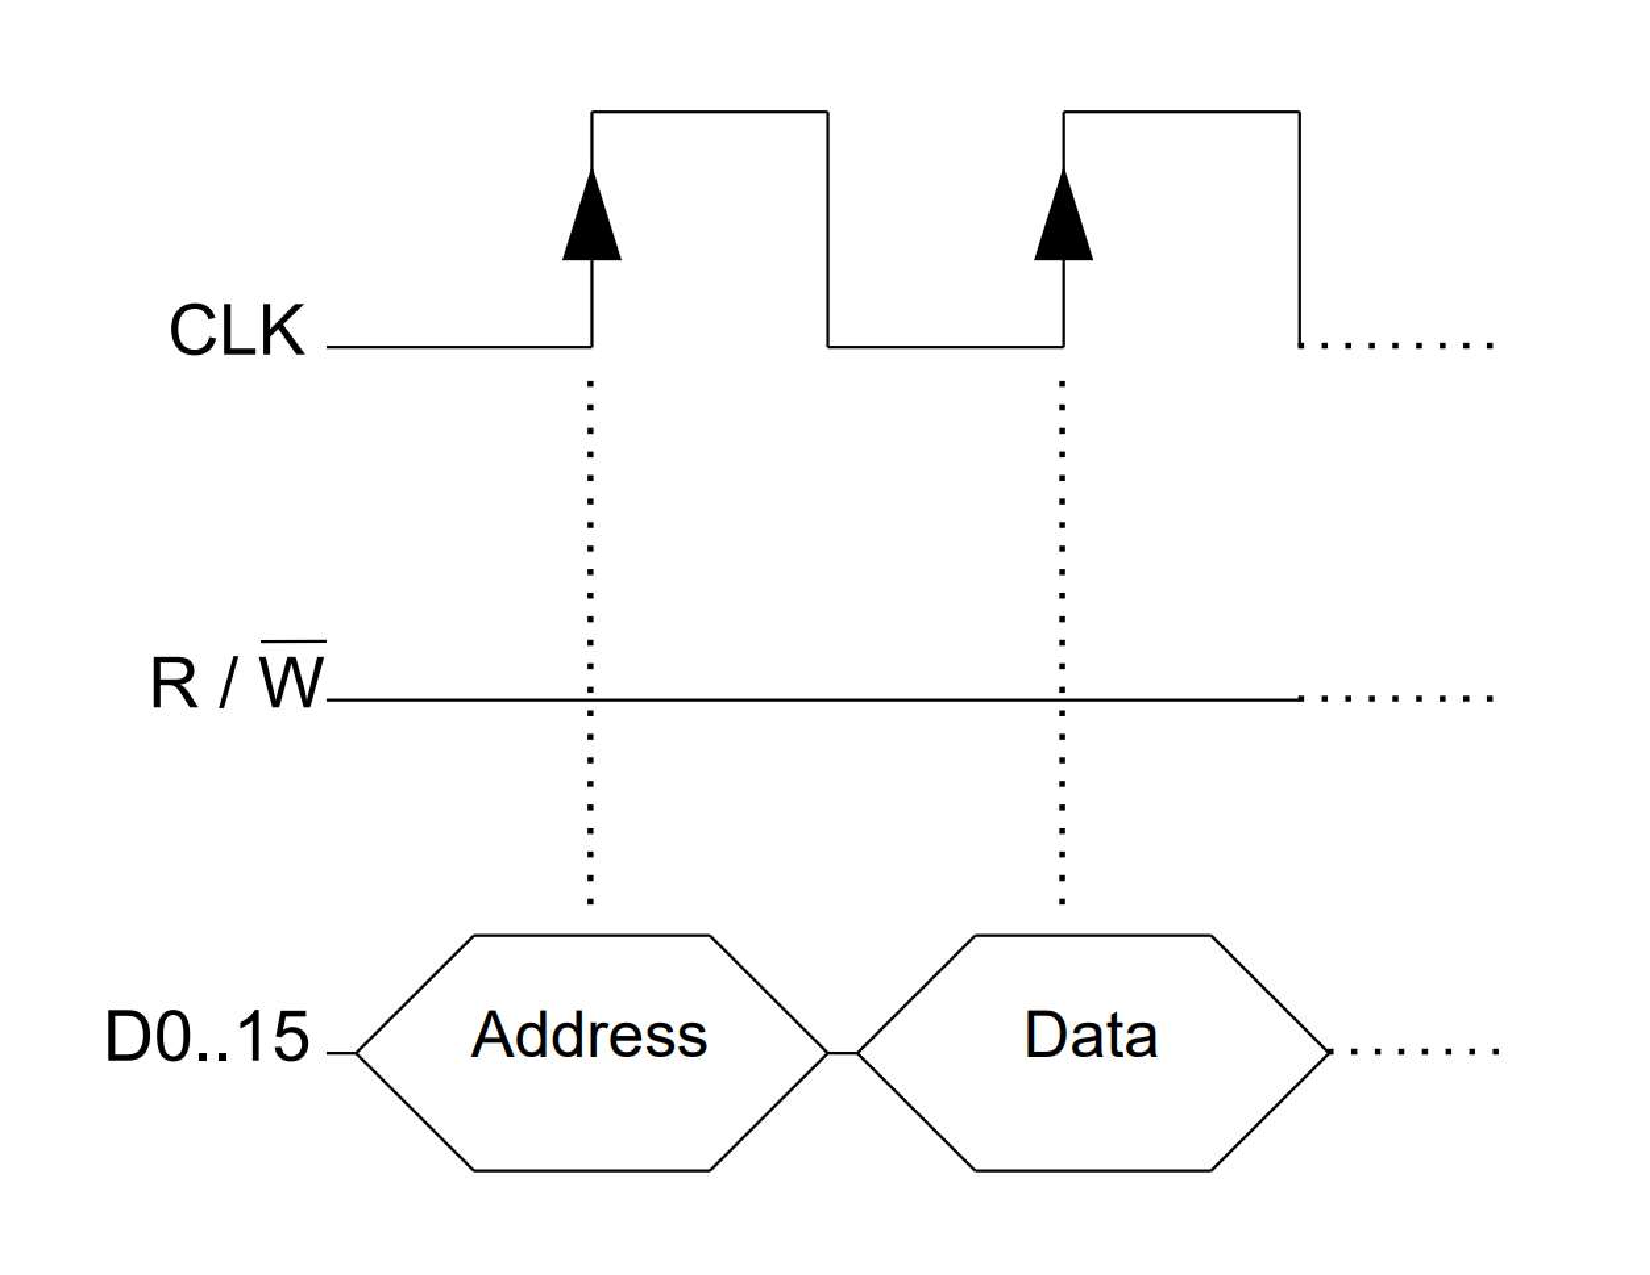
\includegraphics[clip, trim=0 50 0 0, width=0.5\textwidth]{Sections/7_SystemDesign/Figures/7_2_1_CommWrite.pdf}
    \caption{In order to write to the FPGA, the MCU must first set RW ='0' then set the 16 bit bus to the desired address and generate a single CLK pulse. The address is clocked into the FPGA on a rising edge. To write data into the address; the MCU sets 16 bit data on the bus and then generate a single clock pulse. Data is clocked into the FPGA on a rising edge.}
    \label{fig_7_2_1_CommWrite}
\end{figure}

Note how on figure \refq{fig_7_2_1_CommWrite} D0..D15 should have settled before the MCU tries to clock in any value. This will be ensured by design as the signals for the communication are generated sequentially in software on the MCU. They are not hardware controlled and there will be a minimum of \SIQ{35.8}{\nano\second} between D0..D15 and CLK as shown in appendix \refq{App:MicrocontrollerConsiderations} and significantly more if the MCU wants to read from the FPGA.

If the MCU wants to read from the FPGA it must first CLK in an address in the same way as for a write operation, then change it's D0..D15 output pins to input pins and set RW '1'. The following CLK will cause the FPGA to set the data unto the bus pins as shown on figure \refq{fig_7_2_1_CommRead}. \todo{placeholder billede}

\begin{figure}[H]
    \centering
    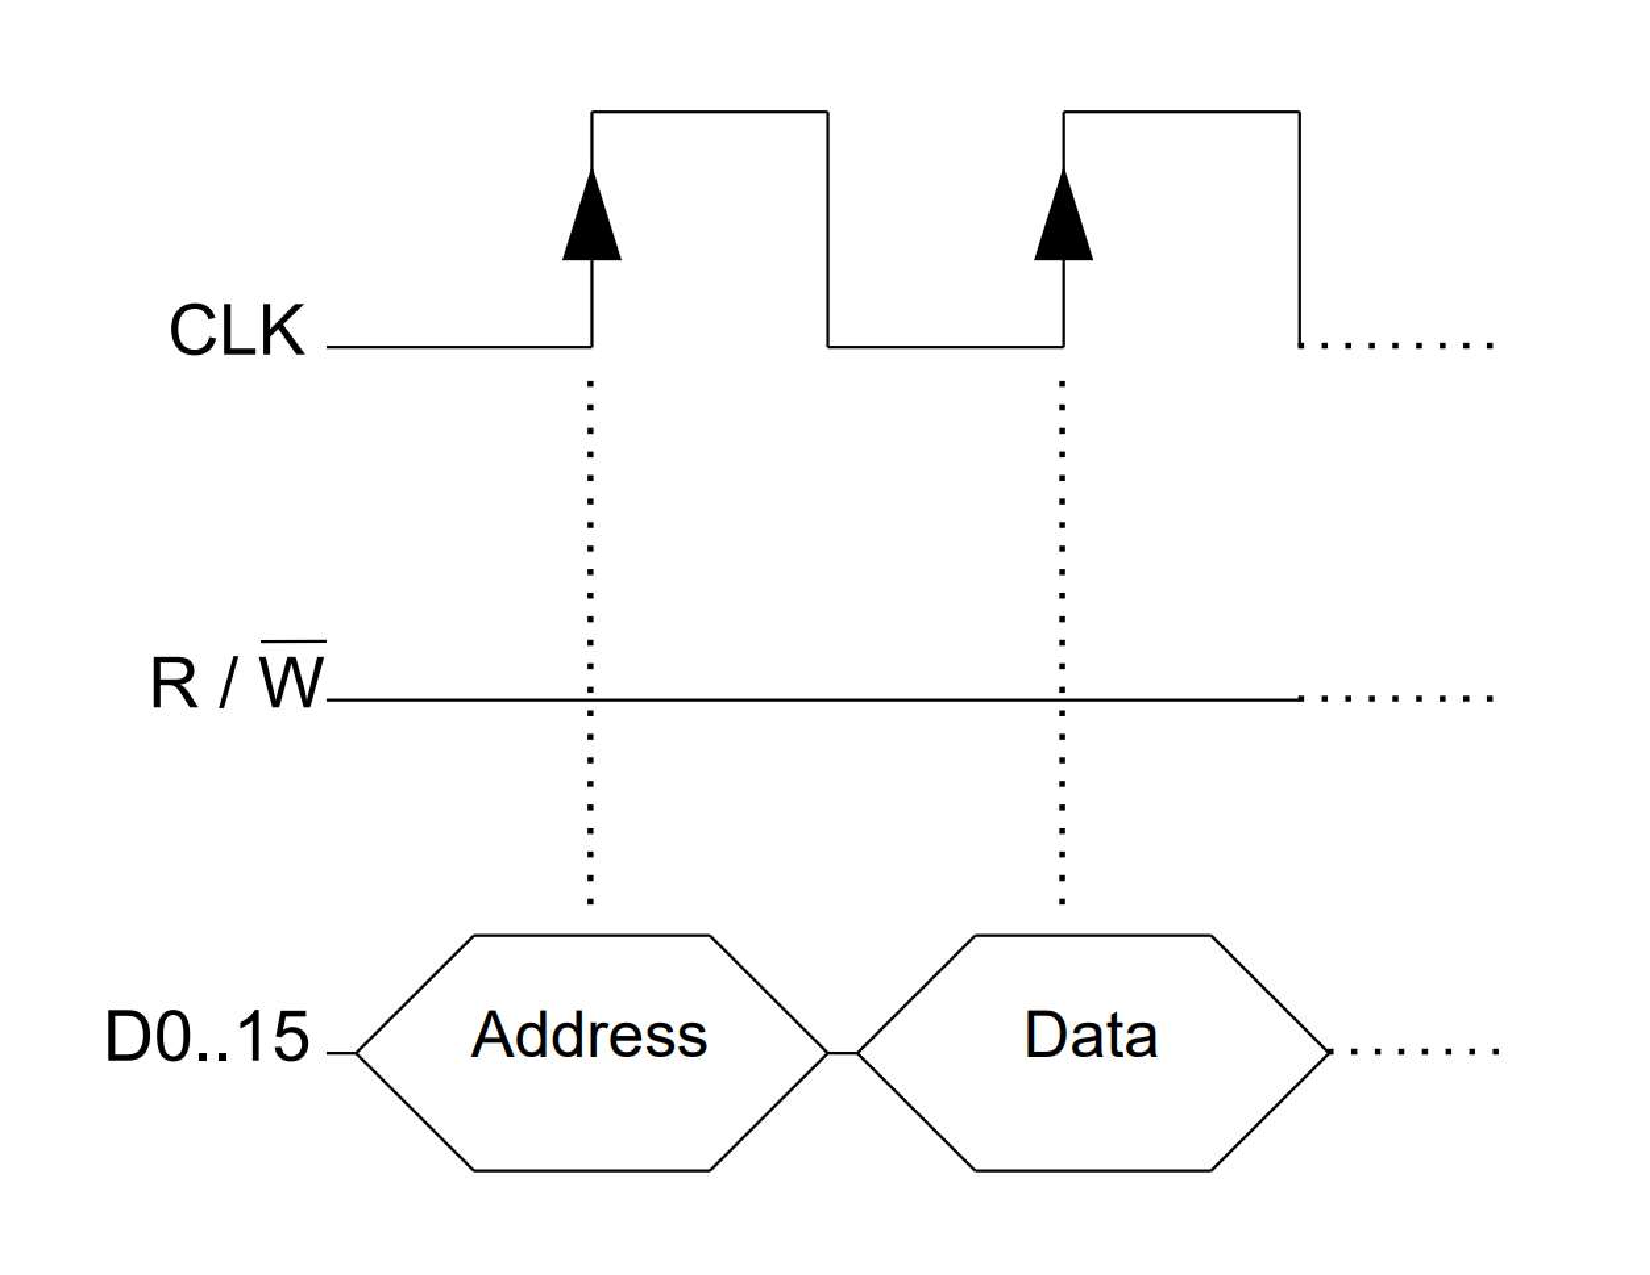
\includegraphics[clip, trim=0 50 0 0, width=0.5\textwidth]{Sections/7_SystemDesign/Figures/7_2_1_CommWrite.pdf}
    \caption{In order to read from the FPGA, the MCU must first set RW ='0' then set the 16 bit bus to the desired address and generate a single CLK pulse. The address is clocked into the FPGA on a rising edge. To read data from the address; the MCU sets RW = '1' and changes it's DB0..DB15 outputs to input. The FPGA clocks the data out on DB0..DB15 on the next rising edge.}
    \label{fig_7_2_1_CommRead}
\end{figure}

The FPGA is using tri-state buffers to function as both inputs and outputs. The Artix 7 FPGA development board is an expensive component and it was decided to let the FPGA use open-drain outputs in order to reduce the risk of both FPGA and MCU actively driving the data bus because of a mistake during development. The logic for this hardware can be seen on listing \refq{lst:7_2_1_CommPort}. 'TOPORT' is data from the internal RAM going to the I/O port and 'TORAM' is data from the I/O going to the RAM.

\lstinputlisting[language=C ,style = c,firstnumber=1, linerange=56-67, caption={VHDL code for the tri-state buffers}, label={lst:7_2_1_CommPort}]{Sections/7_SystemDesign/Code/comm_port.vhd}

The assignment of 'Z' to an 'inout' pin in line 5 will cause the output to enter a high impedance state when it has to produce a logic '1'. This can also be seen on the truth table for the communication port pins as shown on figure \refq{fig_7_2_1_TruthTable}.

\begin{figure}[H]
    \centering
    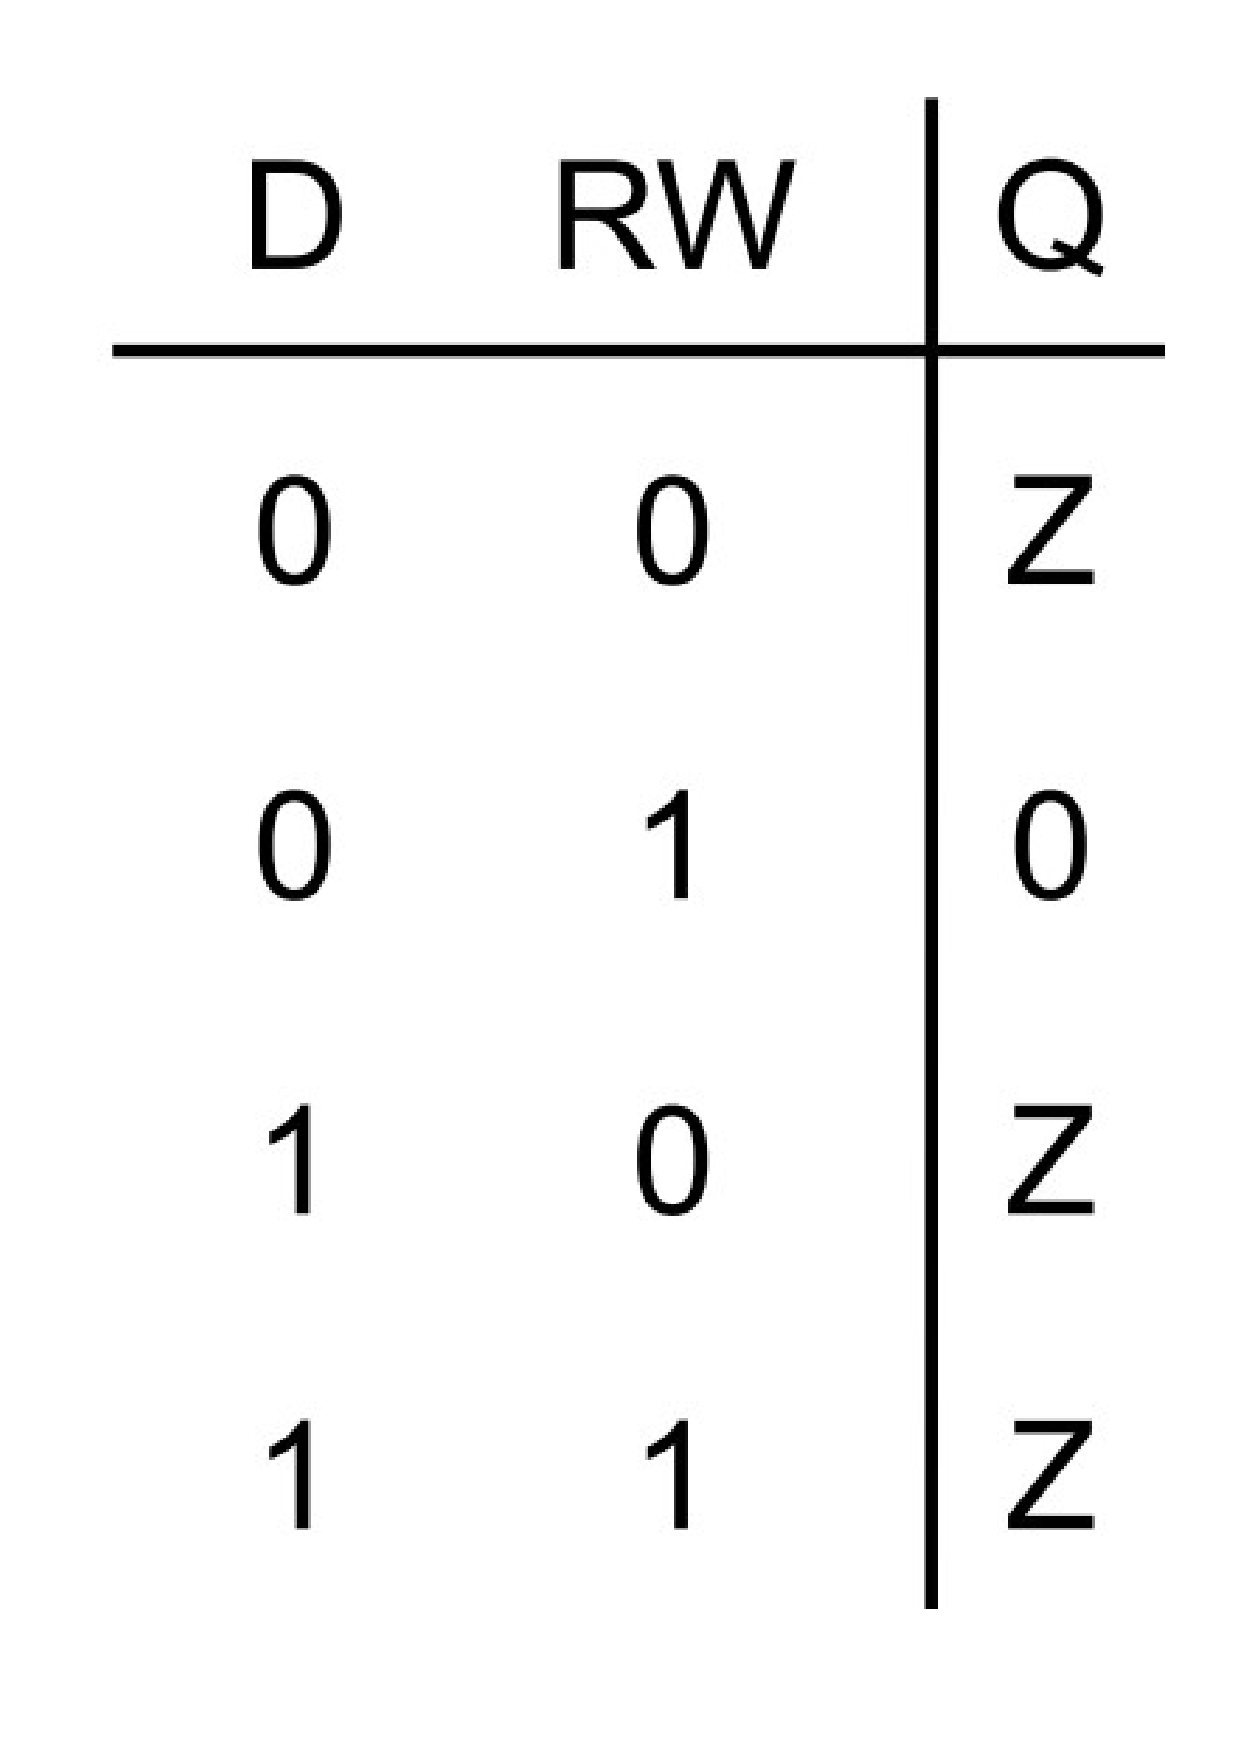
\includegraphics[clip, trim=0 50 0 0, width=0.2\textwidth]{Sections/7_SystemDesign/Figures/7_2_1_IOPortLogic.pdf}
    \caption{A truth table for the input/output port of the FPGA. RW = '0' always puts the port into a high impedance state and RW = '1' lets the port pull the I/O pin to '0'.}
    \label{fig_7_2_1_TruthTable}
\end{figure}

At first glance the I/O port logic on figure \refq{fig_7_2_1_TruthTable} may seem completely useless as it can't output a logic '1'. This is because the I/O pins will require external pull-up resistors in order to produce a '1' when RW = '1'. This will reduce the chance of both FPGA and MCU driving the databus at the same time. The only possible way of damaging the FPGA with the communication bus is if the MCU sets it's output high when RW = '1' and the FPGA sets a '0' as the FPGA pins are high impedance in any other case.

\subsubsection{Communication data rate} \label{subsubsec:CommunicationDatarate}

An estimate of the data rate from this databus can be made based on the findings in appendix \refq{App:MicrocontrollerConsiderations}. For consecutive read operations where the RW signal remains in 'write' mode, the datarate will be limited by the execution time of setting the register in the STM32F446RE. This is also described in appendix \refq{App:MicrocontrollerConsiderations}. From the appendix it takes $t_{clk} = 35.8$ns to toggle the pin by setting and clearing a register and a write to a single register will take $t_{rs} = 17.9$ns. This is useful for calculating the communication throughput.

Every write operation to the RAM requires a 16bit address and 16bit data and two toggles of the CLK. It can be seen in appendix \refq{App:PinMap_MCU_FPGA} on the pin map that the databus on the STM32F446Re is spread over two separate ports, so the MCU will have to write(and read) to two seperate registers in order to write to the FPGA. This is a limitation of the Nucleo development board being used, it would otherwise be possible to do this with a single port, and thus a single register transfer. The total amount of register writes for a single write operation will be as shown in eq \refq{eq:7_2_1_Write_ThroughPut}.

\begin{equation}\label{eq:7_2_1_Write_ThroughPut}
    n_{reg} = n_{clk} +  n_{address} + n_{write} = 4+2+2 = 8 
\end{equation}
It takes a total of 8 register writes to perform a single write operation to the FPGA as shown in equation \refq{eq:7_2_1_Write_ThroughPut}. 4 for toggling the CLK pin twice and 2 each for setting the address and data on the IO pins. Each register write takes \SIQ{17.9}{\nano\second} so the total execution times for a write operation is \SIQ{143.2}{\nano\second} as shown in eq\refq{eq:7_2_1_Write_ThroughPutTotalTime}.
\begin{equation}\label{eq:7_2_1_Write_ThroughPutTotalTime}
    t_{write} = t_{rs} \cdot n_{reg} = 17.9e-9 \cdot 8 =  143.2e-9
\end{equation}
It takes \SIQ{143.2}{\nano\second} for the MCU to perform a write operation. The total throughput on the bus in write mode will be about \SIQ{7}{\mega\bit} as shown in equation \refq{eq:7_2_1_Write_ThroughPut}.

\begin{equation}\label{eq:7_2_1_Write_ThroughPut}
    R_{write} = \frac{1}{t_{write}} = 6.949e6 
\end{equation}
The throughput on the bus is about \SIQ{7}{\mega\bit} in write mode. A significant amount of the throughput is used on protocol overhead as half the transmissions are addresses. The protocol efficiency, $\eta_{p}$, is 
